
% Materials and Methods
%6. Summary of Publication Recommendations
%Published reports must contain sufficient detail to allow other
%experimenters to try to replicate the reported results and to help
%explain failures of replication. Given the limited space that journals
%provide, recommendations will be summarized below for both
%necessary and optional recording and environmental procedures to
%be reported in publications of studies using EDA.
%First and above all, the method of measurement has to be specified:
%endosomatic or exosomatic, direct or alternating current (if
%any) applied to the skin, and constant voltage or constant current.
%The applied voltage (or current) must be noted. If commercially
%available instrumentation has been used, the manufacturer and
%instrument type should be mentioned. Furthermore, calibration
%procedures should be specified.
%Second, methods of signal conditioning and storage need to be
%specified, including procedures for separating EDL from EDRs,
%if applied, time constants of amplifiers, separate grounding procedures,
%if used, A/D conversion rate, and sampling frequency
%(for EDL and EDRs if stored separately).
%Third, recording sites should be specified for active and inactive
%electrodes (if applicable). If the sites were pretreated, the procedure
%should be reported in detail. Also essential is providing details for
%electrodes and electrolytes that were used, such as electrode metal
%(e.g., sintered Ag/AgCl), area of contact (either in square centimeters
%or diameter), method of fixation (e.g., double-sided adhesive
%tape), details of the used electrolyte, such as type of gel or base,
%ionic type and concentration (e.g., 0.08 M or 0.5% NaCl), or, in the
%case of disposable electrodes, brand and type plus as much of the
%above mentioned information as is available from the manufacturer. It is important to know how long electrodes were attached
%before the recording started and how long they stayed in place.
%Details of how polarization was controlled and how electrodes
%were stored should be given if available. In the case of DC recording,
%we recommend using a polarity reversal switch between segments
%within a session.
%Fourth, signal evaluation needs to be reported in detail, whereas
%the sampling rate (for tonic and phasic measures separately, if
%different) and specification of time windows for tonic and phasic
%measures (e.g., latency windows for EDR onset being 1–4 s after
%stimulus onset) are mandatory. For EDRs, a minimum amplitude
%criterion must be specified and reported (e.g., 0.01 mS for SCRs to
%be scored). The standard terminology mentioned in Section 3
%should be adhered to. The term EDR magnitude should be reserved
%for the average amplitude calculated from a series of responses that
%include zero amplitudes. Any treatment of superimposed EDRs
%should be specified. Methods of detection and elimination of
%recording artifacts should be described if applicable.
%Besides the usual details to be reported about procedures for
%laboratory and field settings, it is important for EDA measurement
%to specify baseline conditions in detail, including length and statistical
%treatment during EDAdata evaluation. The gender, age, and
%ethnicity of the participants (e.g., number, range or mean, and
%standard deviation) are essential for comparison with EDA results
%from other studies. Medication or drug use (including caffeine
%intake before participation in the study) need to be reported as well.
%Clothing as well as inside and outside temperatures and their possible
%changes during the recording periods should be reported in as
%much detail as possible. If available (e.g., in case of room airconditioning),
%relative humidity should be reported as well.

\section{Materials and Methods}
% mention the SNNU and the lab where the study takes place
All experiments and measurements were conducted within the facilities of Systems Neuroscience and Neurotechnology Unit, especially the Green Lab, which is located at the Saarland University Hospital. 

\subsection{Participants}


\subsection{Virtual Reality Exposure}
To display the virtual environment, a powerful computer(specs) and a Gainward Nvidia GeForce GTX 1080 Pheonix graphics card with 8 GB of dedicated memory (GDDR5X) were used in combination with the HTC-Vive head-mounted display (HMD). The Dual AMOLED displays (3,6" diagonal) of the HMD provided for a high-resolution presentation of the virtual world,  with 1080x1200 pixel on each eye. The distance between the pupils was manually adjusted for each participant by means of a knob on the HMD. The Lighthouse Tracking-System, created by the company Valve, allowed to track participant's motion during the exposure in an area of maximal 5 by 5 meter and to project their movement in the virtual environment. The Tracking-System consisted of two stationary sensors, positioned in opposing corners at a height of roughly 2 m, and all the sensors, which were attached to the HMD and the controller by HTC. Due to limited space the exposure area was restricted to an area of 3,5 by 3,5 meter. The program, which was used to remotely control the virtual environment, was written with the Matlab software version R2015a. The virtual environment itself was created with Unity version 5.6.1f1 personal. % mention laptop which is used to run the CMU and data presentation

\subsubsection{Virtual Environment}
We have designed our virtual height situation around the concept of a closed room featuring a descending floor. A design, which has been chosen specifically over different approaches that have been used in the past. 

\subsubsection{Closed Loop Setup}
The setup, which was used to conduct the experiment, is composed of three major components, interacting with each other in a closed loop fashion (see figure \ref{setupImg}). The virtual environment is ran on the VR-Unit (VRU) and presented to the subjects through the HMD. Inside the virtual reality the fear triggering stimulus is applied, causing a sympathetic reaction in the subject. This reaction is measured by the bitalino device, in the form of an ECG and GSR signal, and then sent to the control and measurement unit (CMU) via bluetooth. This data is processed by the CMU and displayed, in real-time, for the user to evaluate. Based on the visual input, provided by the CMU, a decision to alter the virtual environment can be made by the user.  

\begin{figure}[ht]
\centering
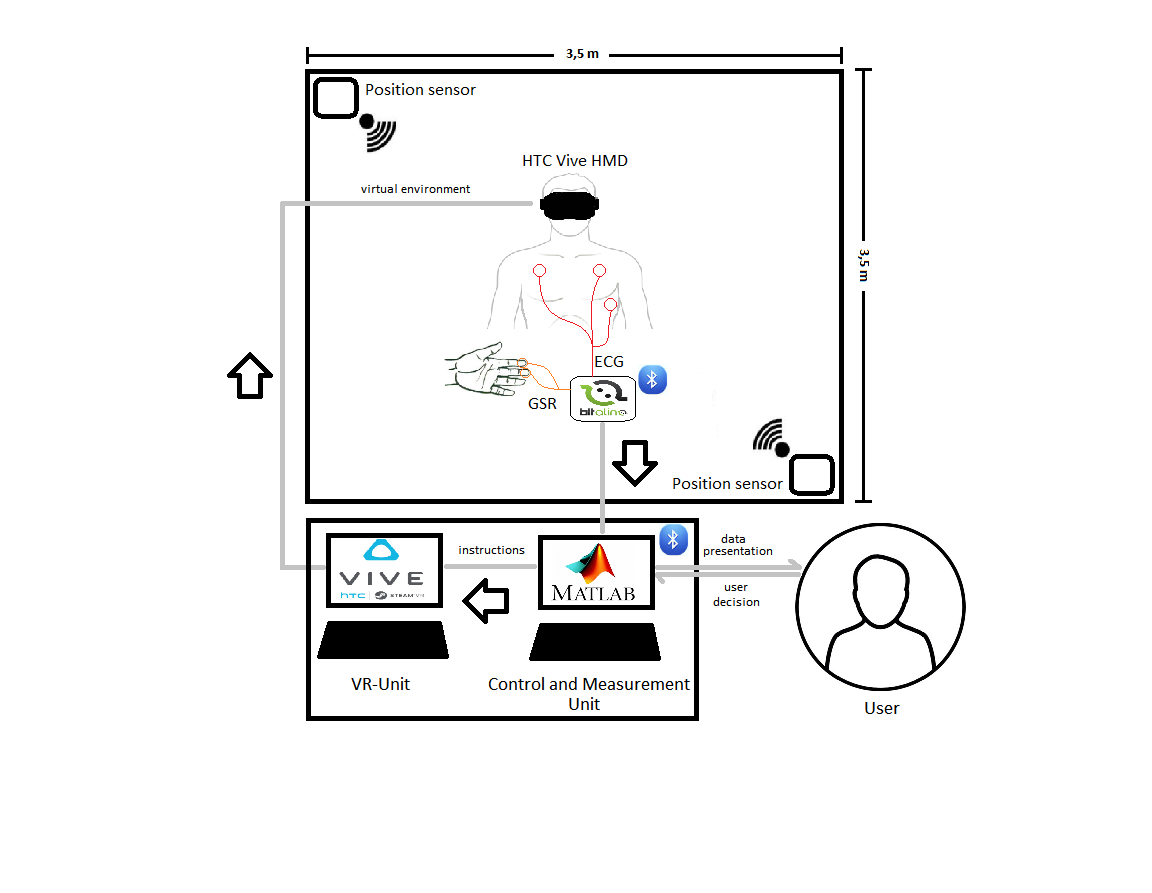
\includegraphics[width=0.8\textwidth]{images/setup.png}
\caption{Closed-loop virtual reality system. The grey line illustrates the closed loop information flow.}
\label{setupImg}
\end{figure}


\subsection{Procedure}
- how many subjects did participate?\\
- which tasks did the patients fullfill? (cross the bridge etc.)\\
- duration of the experiment\\

- description of the virtual environment, the procedure (baseline measurement,VRET in detail)\\ 
- pictures that show the VE in it's starting state as well as it's therapy state (descended floor)\\
- description of how the VR is controlled by the user(which parameters can be influenced)

% methods
- main objective is the measurement of gsr during the therapy and the evaluation of the gsr data concerning the stress of the patient during the therapy\\
- how is the gsr information processed and evaluated?\\
how is it presented to the user?\\
- description of how the VR is controlled by the user(which parameters can be influenced)
- graphic of control chain




-ECG processing frequency domain methods PSD (in task force , reason which method to pick)